\part{Analyse fonctionnelle}

%\sectionmark{}
%\sectionmark{Espaces de Banach et de Hilbert}
\section{Premiers pas avec les espaces de Banach et de Hilbert}
\sectionmark{Premiers pas}

\subsection{Espaces de Banach pour des fonctions continues}
% Sous section 2.1

Notre point de départ sera l'ensemble des fonctions continues $C(I)$ sur un intervalle compact $I := \left[ a,b \right] \subset \mathbb{R}$.

Une manière de déclarer une distance est la \textbf{norme maximale} :
\begin{equation*}
    ||f||_\infty := \max_{x\in I}|f(x)|.
\end{equation*}
Et il devient évident que $C(I)$ devient un espace vectoriel normé.

\begin{definition}
    Un \textbf{espace vectoriel normé $X$} est un espace vectoriel $X$ sur $\mathbb{C}$ (ou $\mathbb{R}$) auquel est associé une fonction positive $||\cdot||:X \rightarrow \mathbb{C}:f \rightarrow ||f||$ telle que
    \begin{enumerate}[label=(\roman*)]
        \item $||f||>0$ pour $f\neq0$ (définie positive),
        \item $||\alpha f|| = |\alpha|\ ||f||$ pour tout $\alpha\in\mathbb{C}$, $f\in X$ (homogénéité positive) et
        \item $||f+g||\leq||f||+||g||$ pour tout $f,g\in X$ (inégalité triangulaire).
    \end{enumerate}
\end{definition}

\begin{remark}
    Soit $(X,||\cdot||)$ un espace vectoriel normé. Alors $(X,d)$ où $d(f,g):=||f-g||$ est un espace métrique.
\end{remark}

Par conséquent, on sait que quand une suite de vecteur $f_n$ converge vers un vecteur $f$ on a $d(f_n,f)\underset{n\to\infty}{\longrightarrow} 0$. On peut donc aussi dire que la suite $f_n$ converge vers $f$ si $||f_n-f|| \underset{n\to\infty}{\longrightarrow} 0$. On écrira alors que $f_n\rightarrow f$ ou $\lim \limits_{n\to\infty} f_n = f$.

\begin{theo}[Inégalité triangulaire inverse]
    \begin{equation*}
        \bigg| ||f||-||g|| \bigg| \leq ||f-g||
    \end{equation*}
\end{theo}

\begin{remark}
    Soit $F:X\rightarrow\mathbb{R}$ avec $X$ un espace métrique. Si $|F(x)-F(\hat x)|\leq d(x,\hat x)$ pour tout $x,\hat x\in X$, alors $F$ est \textit{continue}.
\end{remark}

\begin{theo}
    La fonction $||\cdot||:X\rightarrow\mathbb{R}$ est continue.
\end{theo}

\begin{proof}
    \begin{equation*}
        \bigg| ||f||-||g|| \bigg| \leq ||f-g|| = d(f,g).
    \end{equation*}
\end{proof}

%\begin{theo}
    %La fonction $||\cdot||:X\rightarrow\mathbb{R}$ est connexe.
%\end{theo}

%En plus du concept de convergence, nous avons également le concept d'une \textbf{suite de Cauchy} et par conséquent le concept de complétude : un espace normé est dit \textbf{complet} si chaque suite de Cauchy accepte une limite. Un espace normé complet est appelé \textbf{espace de Banach}.

\begin{definition}
    Un \textbf{espace de Banach} est un espace vectoriel normé complet.
\end{definition}

\begin{example}
    L'espace $l^1(\mathbb{N}) = \{a \in \mathbb{R}^\mathbb{N}:||a||_1<\infty\}$ de toutes les suites de valeurs réelles $a=(a_j)_{j=1}^\infty$ pour lesquelles la norme
    \begin{equation*}
        ||a||_1 := \sum_{j=1}^\infty|a_j|
    \end{equation*}
    est finie est un espace de Banach.
\end{example}

\begin{proof}
    Pour le montrer, nous devons vérifier trois choses : (i) $l^1(\mathbb{N})$ est un espace vectoriel qui est fermé sous addition et multiplication scalaire, (ii) $||\cdot||_1$ satisfait les trois conditions requises d'une norme, et (iii) $l^1(\mathbb{N})$ est complet.\\
    
    (i)$\&$(ii) $\sum \limits_{j=1}^k |a_j+b_j| \leq \sum \limits_{j=1}^k |a_j| + \sum \limits_{j=1}^k |a_j+b_j| \leq ||a||_1 + ||b||_1$ avec $k < \infty$. En faisant tendre $k$ vers l'infini, on observe que l'inégalité triangulaire est satisfaite et que $l^1(\mathbb{N})$ est fermé sous l'addition.
    
    Le fait que la norme 1 est définie positive et satisfait la propriété d'homogénéité positive est direct. Dès lors $l^1(\mathbb{N})$ est fermé sous la multiplication.\\
    
    (iii) Soit $(a^n)_{n\in\mathbb{N}}$ une suite de Cauchy dans $l^1(\mathbb{N})$. Dès lors, $\forall \epsilon>0,\exists N_\epsilon$ tq $||a^m-a^n||_1 \leq \epsilon$ pour $m,n \geq N_\epsilon$.
    
    Donc, pour un nombre $j$ fixé, on a $|a_j^m-a_j^n|\leq\epsilon$ car $|a_j^m-a_j^n| \leq ||a^m-a^n||_1$. Donc la suite $(a^n_j)_{n\in\mathbb{N}}$ est une suite de Cauchy. Or l'ensemble $\mathbb{R} \ni a_j^n$ est complet donc on sait que la suite de Cauchy $(a^n_j)_{n\in\mathbb{N}}$ converge et $\lim \limits_{n\to\infty} a_j^n := a_j$.
    
    Considérons maintenant $\sum \limits_{j=1}^{k} |a_j^m - a_j^n| \leq \epsilon$ avec $m\rightarrow\infty$ : $\sum \limits_{j=1}^{k} |a_j - a_j^n| \leq \epsilon$. Cette inéquation étant valable pour tout $k < \infty$, on a $||a-a^n||_1\leq\epsilon$. Donc $(a-a^n) \in l^1(\mathbb{N})$ et on sait que $a^n \in l^1(\mathbb{N})$ : $a=a^n+(a-a^n) \in l^1(\mathbb{N})$. On conclut donc que la suite $(a^n)_{n\in\mathbb{N}}$ converge vers $a$.
\end{proof}

\begin{example}
    L'exemple précédent peut être généralisé en considérant l'espace $l^p(\mathbb{N})$ de toutes les suites de valeurs complexes $a=(a_j)_{j=1}^\infty$ pour lesquelles la norme $p \in [1,\infty[$ est est finie.
    \begin{figure}[H]
        \centering
        \tikzsetnextfilename{produit_cartesien} 
        \begin{tikzpicture}
            \draw[->] (0,-.5) -- (0,2.5);
            \draw[->] (-.5,0) -- (4,0);
            \draw plot[mark=*, mark size=.3mm] (.5,0) -- plot[mark=*, mark size=.3mm] (.5,2) node[above] {$a_1$};
            \draw plot[mark=*, mark size=.3mm] (1,0) -- plot[mark=*, mark size=.3mm] (1,-.6) node[below] {$a_2$};
            \draw plot[mark=*, mark size=.3mm] (1.5,0) -- plot[mark=*, mark size=.3mm] (1.5,.4)  node[above] {$a_3$};
            \draw plot[mark=*, mark size=.3mm] (2,0) -- plot[mark=*, mark size=.3mm] (2,1.3) node[above] {$a_4$};
            \draw (3,0) node[below] {$\cdots$};
            \draw (-.5,1) node[left] {$l^p(\mathbb{N}) \ni$};
            \draw (6,1) node[right] {$||a||_p := \left(\sum|a_n|^p\right)^{1/p} < \infty$};
            
            \draw[->] (0,-4) -- (0,-1);
            \draw[->] (-.5,-2.5) -- (4,-2.5);
            \draw plot[mark=*, mark size=.3mm] (.5,-2.5) -- plot[mark=*, mark size=.3mm] (.5,-2);
            \draw plot[mark=*, mark size=.3mm] (1,-2.5) -- plot[mark=*, mark size=.3mm] (1,-1.5);
            \draw plot[mark=*, mark size=.3mm] (1.5,-2.5) -- plot[mark=*, mark size=.3mm] (1.5,-3.2);
            \draw plot[mark=*, mark size=.3mm] (2,-2.5) -- plot[mark=*, mark size=.3mm] (2,-2.8);
            \draw[dashed] (-.5,-1.5) -- (3.8,-1.5) node[right] {$||a||_\infty$};
            \draw[dashed] (-.5,-3.5) -- (3.8,-3.5) node[right] {$-||a||_\infty$};
            \draw (3,-2.5) node[below] {$\cdots$};
            \draw (-.5,-2.5) node[left] {$l^\infty(\mathbb{N}) \ni$};
            \draw (6,-2.5) node[right] {$||a||_\infty := \mathrm{sup}_{n\in\mathbb{N}} |a_n|_{<\infty}$};
        \end{tikzpicture}
    \end{figure}
\end{example}

\begin{figure}[H]
    \centering
    \includegraphics[scale = .5]{unitball.png}
    \caption{Balle unité pour $||\cdot||_p$ dans $\mathbb{R}$}
    \label{fig:unitball}
\end{figure}

\begin{remark}
    La norme $p$ avec $p \in [0,1[$ n'est pas une norme car l'inégalité triangulaire n'est pas satisfaite.
\end{remark}

\begin{remark}
    Toute norme est une fonction CONVEXE. On observe bien sur la figure \ref{fig:unitball} que la fonction $\{a:||a||_{p=0.5}\}$ est concave et que $\{a:||a||_{p\geq1}\}$ sont convexes.
\end{remark}

\vspace{0.5cm}
Du coup, quid de la \textbf{complétude de $C(I)$} ?
%Une suite de fonctions $f_n(x)$ converge vers $f$ si et seulement si
%\begin{equation}
    %\lim_{n\rightarrow \infty}||f-f_n||_\infty = \lim_{n\rightarrow \infty}\sup_{x\in I}|f(x) - f_n(x)| = 0 \qquad \text{(on s'intéresse à $C(I)$ muni de la norme $||\cdot||_\infty$)}.
%\end{equation}
%Maintenant, ayant en tête le cas où $f_n$ est une suite de Cauchy seulement. Alors $f_n(x)$ est une suite de Cauchy de nombres complexes pour tout $x\in I$ fixé. En particulier, par complétude de $\mathbb{C}$, il existe une limite $f(x)$ pour chaque $x$. On obtient donc une fonction $f(x)$ limitée et quand $m\rightarrow\infty$, on voit que l'inégalité de Cauchy se transforme :
%\begin{equation}
    %|f(x)-f_n(x)|\leq\epsilon \quad \forall n>N_\epsilon,\ x\in I.
%\end{equation}

\begin{theo}
    $C(I)$ avec une norme maximale est un espace de Banach.
\end{theo}

\begin{proof}
    \begin{enumerate}[label=(\roman*)]
        \item Comme $C(I)$ est stable par combinaison linéaire, il est un espace vectoriel.
        \item $||f||_\infty := \max_{x\in I}|f(x)|$ est bien défini (Théorème \ref{theo:valextr}) et satisfait les propriétés de la norme.
        \item $C(I),\ ||\cdot||_\infty$, est complet ; soit $(f_n)_{n\in\mathbb{N}}$ une suite de Cauchy dans $C(I)$, c'est-à-dire
        \begin{align*}
            \lim_{m,n\rightarrow\infty} ||f_n-f_m||_\infty & = \lim_{m,n\rightarrow\infty} \max_{x\in I} |f_n(x) - f_m(x)| = 0 \nonumber\\
            \iff \lim_{m,n\rightarrow\infty} |f_n(x) - f_m(x)| & \leq \lim_{m,n\rightarrow\infty} \max_{x\in I} |f_n(x) - f_m(x)| = 0 \nonumber \\
            %\lim_{m,n\rightarrow\infty} ||f_n-f_m||_\infty & = 0.
        \end{align*}
        C'est-à-dire que pour tout $x$ fixé dans $I$, $f_n(x)$ est une suite de Cauchy dans $\mathbb{R}$ (espace \textit{complet}). Donc $[f_n(x)]_{n=1}^\infty \in \mathbb{R}$ a une $\lim := f(x)$. \\ Vu que $f_n\ (\in C(I))$ est de Cauchy :
        \begin{align*}
            \forall\epsilon>0,\exists N_\epsilon:\forall m,n>N_\epsilon & : ||f_n-f_m||_\infty\leq\epsilon \\
            \forall\epsilon>0,\exists N_\epsilon:\forall m,n>N_\epsilon,\forall x\in I & : |f_n(x)-f_m(x)|\leq\epsilon \\
            \forall\epsilon>0,\exists N_\epsilon:\forall x\in I:\forall n>N_\epsilon:\forall m>N_\epsilon & : |f_n(x)-f_m(x)|\leq\epsilon \\
            \forall\epsilon>0,\exists N_\epsilon:\forall x\in I:\forall n>N_\epsilon & : \lim \limits_{m\to\infty} |f_n(x)-f_m(x)|\leq\epsilon \\
            \forall\epsilon>0,\exists N_\epsilon:\forall x\in I:\forall n>N_\epsilon & : |f_n(x)-f(x)|\leq\epsilon \\
            \forall\epsilon>0,\exists N_\epsilon:\forall n>N_\epsilon:\forall x\in I & : |f_n(x)-f(x)|\leq\epsilon\\
            \forall\epsilon>0,\exists N_\epsilon:\forall n>N_\epsilon & : ||f_n-f||_\infty\leq\epsilon.
        \end{align*}
        C'est-à-dire que $f_n$ converge uniformément vers $f$, et donc que $f_n$ converge vers $f$ au sens de $||\cdot||_\infty$. \\
        Il reste à montrer que $f\in C(I)$ (autrement dit que $f$ est continue sur l'intervalle $I$), ce qui est vrai puisque la limite uniforme de fonctions continues est continue :
        \begin{equation*}
            |f(x)-f(y)| \leq \underbrace{|f(x)-f_n(x)|}_{\leq \frac{\epsilon}{3}} + \underbrace{|f_n(x)-f_n(y)|}_{\leq \frac{\epsilon}{3} \text{ car $f_n$ continue}} + \underbrace{|f_n(y)-f(y)|}_{\leq \frac{\epsilon}{3}} \leq \epsilon.
        \end{equation*}
    \end{enumerate}
\end{proof}

\begin{definition}[Delta de Kronecker]
    \begin{equation*}
        \delta_{n,m} := \left\{ \begin{array}{ll}
            1 & \mathrm{si}\ n=m \\
            0 & \mathrm{sinon}
        \end{array} \right.
    \end{equation*}
    \begin{equation*}
        \delta^n := \left( \delta_{n,m} \right)_{m\in\mathbb{N}}\in l^p(\mathbb{N}),\ p\in [1,\infty)
    \end{equation*}
\end{definition}

\begin{definition}
    Soit $\{u_n\}_{n\in\mathcal{N}}\subset X$. Le \textbf{sous-espace vectoriel} engendré par la suite est l'ensemble des combinaisons linéaires finies des $\{u_n\}_{n\in\mathcal{N}}$, c'est-à-dire :
    \begin{equation*}
        \mathrm{span}\{u_n\}_{n\in\mathcal{N}} := \left\{\sum_{j=1}^m \alpha_j u_{n_j} \Big | n_j\in\mathcal{N}, \alpha_j\in\mathbb{R},m\in\mathbb{N} \right\}
    \end{equation*}
\end{definition}

\begin{example}
    $\mathrm{span}\{ \delta^1, \delta^2, \cdots \} = \left\{ a\in l^p(\mathbb{N}) \big | \sup(a)<\infty \right\}$
\end{example}

\begin{definition}
    $\{u_n\}_{n\in\mathcal{N}}$ est \textbf{linéairement indépendant} si tout sous-ensemble fini de cette suite est linéairement indépendant.
\end{definition}

\begin{definition}
    Un (sous-)ensemble (de $X$, un espace vectoriel normé) est \textbf{total} si son ``span'' est dense (dans $X$).
\end{definition}

\begin{definition}
    Un espace vectoriel normé $X$ est \textbf{séparable} s'il contient un ensemble dense et dénombrable. (même chose que les espaces métriques...)
\end{definition}

\begin{theo}
    Si $X$ contient un ensemble total dénombrable, alors $X$ est séparable
\end{theo}

\begin{proof}
    Soit $\{u_n\}_{n\in\mathbb{N}}$ total. On a :
    \begin{equation*}
        \mathrm{span}\{u_n\}_{n\in\mathbb{N}} = \left\{ \sum_{j=1}^m \alpha_j u_{n_j} \Big | n_j\in\mathbb{N}, \alpha_j\in Q,m\in\mathbb{N} \right\}
    \end{equation*}
    où $Q$ est dense et $m\in \mathbb{N}$ est dénombrable.
\end{proof}

\begin{example}
    Pour $p \in [1,\infty[$, l'ensemble $\{\delta^1,\delta^2,...\}$ est total (dans $l^p(\mathbb{N})$) et dénombrable donc $l^p(\mathbb{N})$ est séparable.
\end{example}

\begin{proof}
    Soit $a = (a_j)_{j\in\mathbb{N}} \in l^p(\mathbb{N})$. Alors, $\big[||a-\sum \limits_{n=1}^m a_n \delta^n||_p\big]^p = \sum \limits_{n=m+1}^\infty |a_n|^p$ car $a_j^m = a_j$ pour $j \in [1,m]$ et $a_j^m = 0$ pour $j>m$. Donc, $\sum \limits_{n=m+1}^\infty |a_n|^p = \big[||a||_p - \sum \limits_{n=1}^m |a_n|\big]^p \rightarrow 0$ parce que $\lim \limits_{m\to\infty} \sum \limits_{n=1}^m |a_n| = ||a||_p$. Donc $\{\delta^1,\delta^2,...\}$ est total et $l^p(\mathbb{N})$ est séparable.
\end{proof}

\begin{remark}
    L'ensemble $l^\infty(\mathbb{N})$ est non séparable (démo TP6).
\end{remark}

\begin{lemme}[Lissage] \label{lem:lissage}
    Soit $u_n$ une suite de fonctions continues non négatives sur $[-1;1]$ telle que pour tout $\delta>0$,
    \begin{equation*}
        \int_{-1}^1 u_n(x)\ dx = 1 \quad\mathrm{et}\quad \int_{\delta\leq|x|\leq1} u_n(x)\ dx \underset{n\to \infty}{\rightarrow} 0.
    \end{equation*}
    (En d'autres mots, $u_n$ a une masse égale à 1 et tend vers la valeur nulle quand $n\to\infty$).
    
    Alors, pour tout $f\in C\left[ -\frac{1}{2},\frac{1}{2} \right]$ qui s'annule aux extrémités : $f\left(-\frac{1}{2}\right) = f\left(\frac{1}{2}\right) = 0$, on a que
    \begin{equation*}
        f_n(x) := \int_{-\frac{1}{2}}^\frac{1}{2} u_n(x-y)f(y)\ dy
    \end{equation*}
    converge uniformément vers $f(x)$.
\end{lemme}
%\begin{proof}
    %Comme $f$ est uniformément continue, on peut trouver pour un $\epsilon$ donné un $\delta<\frac{1}{2}$ (indépendant de $x$) tel que $|f(x)-f(y)|\leq\epsilon$ quand $|x-y|\leq\delta$. De plus, on peut choisir $n$ tel que $\int_{\delta\leq|y|\leq1} u_n(y)dy\leq\epsilon$. Abrégeons maintenant $M = \max_{x\in\left[ -\frac{1}{2},\frac{1}{2} \right]}\{1,|f(x)|\}$ et notons
    %\begin{equation*}
        %\left| f(x) - \int_{-\frac{1}{2}}^\frac{1}{2} u_n(x-y)f(x)\ dy \right| = |f(x)|\ \left| 1 - \int_{-\frac{1}{2}}^\frac{1}{2} u_n(x-y)\ dy \right|\leq M\epsilon.
    %\end{equation*}
    %Il revient en fait au même de dire que la distance de $x$ aux points frontières est plus petite que $\delta$ et par conséquent $|f(x)|\leq\epsilon$ ou que $[-\delta,\delta]\subset[x-1/2,x+1/2]$ et le différence de 1 avec l'intégrale est plus petite que $\epsilon$. \\
    %On a alors
    %\begin{align*}
        %|f_n(x) - f(x)| & \leq \int_{-\frac{1}{2}}^\frac{1}{2} u_n(x-y)|f(y)-f(x)|dy + M\epsilon \nonumber \\
                        %& = \int_{|y|\leq1/2,|x-y|\leq\delta} u_n(x-y) |f(y) - f(x)|dy + \int_{|y|\leq1/2,|x-y|\geq\delta} u_n(x-y) |f(y) - f(x)|dy + M\epsilon \nonumber \\
                        %& \leq \epsilon + 2M\epsilon + M\epsilon = (1+3M)\epsilon.
    %\end{align*}
%\end{proof}

\begin{theo}[Weierstrass]
    L'ensemble des polynômes est dense dans $\left(C(I), ||\cdot||_\infty\right)$ pour tout intervalle $I$ compact.
\end{theo}
\begin{proof}
    Soit $f\in C(I)$. Prenons $I=\left[ -\frac{1}{2},\frac{1}{2} \right]$ sans perte de généralité. Supposons aussi que $f\left(-\frac{1}{2}\right) = f\left(\frac{1}{2}\right)=0$. Utilisons le lemme précédent avec
    \begin{equation*}
        u_n(x) = \frac{1}{I_n} (1-x^2)^n
    \end{equation*}
    avec 
    \begin{equation*}
        I_n = \int_{-1}^1 (1-x^2)^n\ dx = \frac{n!}{\frac{1}{2}\left(\frac{1}{2}+1\right)\cdots\left(\frac{1}{2}+n\right)}
    \end{equation*}
    afin que $\int_{-1}^1 u_n \ dx = 1$ ($u_n$ décroît très rapidement).
    
    Dès lors,
    \begin{equation*}
        \frac{1}{\frac{1}{2}+n} < I_n < 2.
    \end{equation*}
    Comme $u_n(x)$ est continue non-négative sur $[-1,1]$, que son intégrale sur ce domaine est égale à 1, on montre finalement
    \begin{equation*}
        \int_{\delta\leq|x|\leq1}u_n(x)dx \leq 2(1-\delta)u_n(\delta) \leq 2u_n(\delta) = \frac{2(1-\delta^2)^n}{I_n} = (1+2n)(1-\delta^2)^n \underset{n\to\infty}{\longrightarrow} 0.
    \end{equation*}
    
    Les hypothèses du lemme de lissage sont satisfaites donc $f_n(x) = \int_{\frac{-1}{2}}{\frac{1}{2}} u_n(x-y)f(y)\ dy$ converge uniformément vers $f(x)$ : $||f-f_n|| \underset{n\to\infty}{\longrightarrow} 0$
\end{proof}

\textbf{Corollaire :} Les monômes $(1,x,x^2,...)$ sont totaux dans $C(I),||\cdot||_\infty$ et donc $C(I)$ est séparable.

\subsection{La géométrie des espaces de Hilbert}
% Sous-section 2.2

\begin{definition}
    Un \textbf{produit scalaire} sur un espace vectoriel réel $X$ est une application $\langle\cdot,\cdot\rangle:X\times X\rightarrow\mathbb{R}$ telle que
    \begin{enumerate}
        \item $\langle u,u \rangle>0$ pour tout $u\in X\setminus\{0\}$ (définie positive);
        \item $\langle \alpha u + \beta v,w \rangle = \alpha\langle u,w \rangle + \beta\langle v,w \rangle$ pour tous $\alpha,\beta\in\mathbb{R}$ et $u,v\in X$ (application bilinéaire);
        \item $\langle u,v \rangle = \langle v,u \rangle$ pour tous $u,v\in X$ (symétrique).
    \end{enumerate}
\end{definition}

\begin{remark}
    Dans les complexes la propriété de bilinéarité est un peu plus compliquée. Supposons que $\mathcal{H}$ soit un espace vectoriel. Une relation $\langle\cdot,\cdot\rangle = \mathcal{H}\times\mathcal{H} \rightarrow\mathbb{C}$ est appelée \textbf{forme sesquilinéaire} si
    \begin{equation*}
        \begin{array}{rcl}
            \langle \alpha_1f_1 + \alpha_2f_2,g \rangle & = & \alpha_1^\star\langle f_1,g \rangle + \alpha_2^\star \langle f_2,g \rangle, \\
            \langle f,\alpha_1g_1 + \alpha_2g_2 \rangle & = & \alpha_1\langle f,g_1 \rangle + \alpha_2 \langle f,g_2 \rangle,
        \end{array}
        \alpha_1,\alpha_2\in\mathbb{C},
    \end{equation*}
    où `$\star$' dénote le complexe conjugué. Une forme sesquilinéaire symétrique ($\langle f,g \rangle = \langle g,f \rangle^\star$) est appelée \textbf{forme hermitienne} et un produit scalaire défini dans les complexes est donc une forme hermitienne définie positive ($\langle f,f \rangle>0$ pour $f\neq0$).
\end{remark}

\begin{definition}
    Un \textbf{espace préhilbertien} ou \textbf{à produit scalaire} est un espace vectoriel muni d'un produit scalaire.
\end{definition}

\begin{remark}
     D'un produit scalaire découle toujours une norme et $||f|| = \sqrt{\langle f,f \rangle}$. On peut aussi définir une distance : $d(f,g) = ||f-g||$.
     
     \danger Une norme ne provient pas toujours d'un produit scalaire
\end{remark}

\begin{definition}
    Un \textbf{espace de Hilbert} est un espace préhilbertien complet.
\end{definition}

\begin{example}
    Soit l'espace de Hilbert $l^2(\mathbb{N})$, l'ensemble composé des suites complexes :
    \begin{equation*}
        \left\{ a = (a_j)_{j=1}^\infty\in\mathbb{N} \bigg| ||a||_2^2 = \sum_{j=1}^\infty |a_j|^2 < \infty \right\}.
    \end{equation*}
    Ile faut prouver que cette norme est induite par un produite scalire. Soit le produit scalaire $\langle a,b \rangle := \sum_{j=1}^\infty a_j^\star b_j$, c'est une série et il faut prouver qu'elle converge. Par l'inégalité de Cauchy-Schwarz (théorème \ref{theo:Cauchy-Schwarz}), on déduit
    \begin{equation*}
        \left|\sum_{j=1}^n a_j^\star b_j\right|^2 \leq \sum_{j=1}^n |a_j|^2 \sum_{j=1}^n |b_j|^2.
    \end{equation*}
    La somme définie dans le produit scalaire est donc absolument convergente pour $a,b\in l^2(\mathbb{N})$. Observons que la norme $||a||=\sqrt{\langle a,a \rangle}$ est identique à la norme $||a||_2$ définie précédemment. En particulier $l^2(\mathbb{N})$ est complet pour la norme 2 et donc c'est un espace de Hilbert.
\end{example}

\begin{definition}
    $f,g\in\mathcal{H}$ sont \textit{orthogonaux} si $\langle f,g \rangle = 0.$
\end{definition}

\begin{definition}
    $f,g\in\mathcal{H}$ sont \textit{parallèles} s'ils sont multiples l'un de l'autre : $ f = ag$, $a\in\mathbb{R}$.
\end{definition}

\begin{theo}[Pythagore]
    Si $f\bot g$ alors $||f+g||^2 = ||f||^2 + ||g||^2$. \label{theo:pythagore}
\end{theo}

\begin{remark}
    $f_\sslash$ est la projection de $f$ sur $\mathbb{R}u$ où $\mathbb{R}u = \text{span}(\{u\}):= \{\alpha u | \alpha\in\mathbb{R}\}$ : $f_\sslash$ est le point de $\text{span}(\{u\})$ le plus proche de $f$ au sens de la norme induite.
\end{remark}
\begin{proof}
    Soit $u,f\in\mathcal{H}$ tels que $||u||=1$ et $f = f_{\sslash} + f_\bot$ tels que $f_{\sslash}\sslash u$, $f_\bot \bot u$. On a donc
    \begin{center}
        \begin{minipage}{0.3\textwidth}
            \begin{align*}
                f_{\sslash} &:= \langle u,f \rangle u, \\
                f_{\bot}    &:= f - \langle u,f \rangle u.
            \end{align*}
        \end{minipage}
        \begin{minipage}{0.3\textwidth}
            \centering
            \includegraphics[scale = 0.5]{synthese_projection.PNG}
        \end{minipage}
    \end{center}
    
    On vérifie alors que
    \begin{equation*}
        \langle u,f_{\bot} \rangle = \langle u,f - \langle u,f \rangle u \rangle = \langle u,f \rangle - \langle u,f \rangle \langle u,u \rangle = 0.
    \end{equation*}
    Prenons n'importe quel autre vecteur $\alpha u$ parallèle à $u$. En utilisant \ref{theo:pythagore}, on obtient alors
    \begin{equation*}
        ||f-\alpha u||^2 = ||f_\bot + (f_\sslash - \alpha u)||^2 = ||f_\bot + (\langle u,f \rangle u - \alpha u)||^2 = ||f_\bot||^2 + |\langle f,u \rangle - \alpha|^2 ||u||^2 = ||f_\bot||^2 + |\langle f,u \rangle - \alpha|^2.
    \end{equation*}
    On trouve donc que $||f-\alpha u||$ est minimal pour $\alpha = \langle f,u \rangle$.
\end{proof}

\begin{theo}[Cauchy-Schwarz]
    Soit $\mathcal{H}$ un espace vectoriel à produit scalaire. Pour tout $f,g\in\mathcal{H}$
    \begin{equation*}
        \left|\langle f,g \rangle\right| \leq ||f||\ ||g||.
    \end{equation*}
    On parle alors de norme induite. (il y a égalité si $f$ et $g$ sont parallèles).
    \label{theo:Cauchy-Schwarz}
\end{theo}

\begin{proof}
    Commençons par le cas le plus trivial où $g=0$. On a alors $\left|\langle f,g \rangle\right| = ||f||\ ||g|| = 0$ et la proposition est vérifiée. Supposons maintenant que $g$ soit non nul et définissons le vecteur unitaire $u$ par
    \begin{equation*}
        u := \frac{g}{||g||}.
    \end{equation*}
    On cherhce alors à montrer que
    \begin{equation*}
        \left|\langle f,u \rangle\right| \leq ||f||
    \end{equation*}
    ce qui est correct puisque
    \begin{equation*}
        ||f||^2 = ||f_\sslash||^2 + ||f_\bot||^2 = \left|\langle f,u \rangle\right|^2 + ||f_\bot||^2.
    \end{equation*}
\end{proof}

Le théorème de Cauchy-Schwarz a pour conséquence que
\begin{itemize}
    \item $\mathcal{H}\times\mathcal{H}\to\mathbb{R}:f,g\to\langle f,g \rangle$ est continue ;
    \item $||\cdot|| = \sqrt{\langle\cdot,\cdot\rangle}$ satisfait bien l'inégalité du triangle.
\end{itemize}

\begin{theo}[Jordan-von Neumann]
    Soit $||\cdot||$ une norme. Il existe alors un produit scalaire $\langle\cdot,\cdot\rangle$ tel que $||\cdot|| = \sqrt{\langle\cdot,\cdot\rangle}$ ssi $\forall f,g$ :
    \begin{equation*}
        ||f+g||^2 + ||f-g||^2 = 2||f||^2 + 2||g||^2 \quad\mathrm{(r\Grave{e}gle\ du\ parall\Acute{e}logramme)}
    \end{equation*}
    Dans ce cas, on peut retrouver le produit scalaire par la définition de la norme :
    \begin{equation*}
        \langle f,g \rangle = \frac{||f+g||^2 - ||f-g||^2}{4}
    \end{equation*}
\end{theo}

Rappelons que notre but initial était d'obtenir un produit scalaire sur $C(I)$. On peut définir un tel produit sur $I=[a,b]$ par
\begin{equation*}
    \langle f,g \rangle := \int_a^b f(x)g(x)\ dx
\end{equation*}
La relation vérifie les 3 propriétés du produit scalaire.

\begin{definition}
    $\mathcal{L}_{cont}^2(I)$ est un espace préhilbertien : c'est l'ensemble $C(I)$ muni du produit scalaire définit ci-dessus.
\end{definition}

\begin{remark}
    Les ensembles $\mathcal{L}_{cont}^2(I)$ et $C(I)$ ne diffèrent que par la norme qui leur est attribué. En effet, à $\mathcal{L}_{cont}^2(I)$ on associe la norme induite alors qu'à $C(I)$ est associé la norme infinie.
\end{remark}

\begin{definition}
    On définit par $||f||_2$ la norme de $f$ dans $\mathcal{L}_{cont}^2(I)$ :
    \begin{equation*}
        ||f||_2 = \sqrt{\int_a^b |f(x)|^2 dx} \neq ||f||_\infty.
    \end{equation*}
\end{definition}

\begin{definition}
    $||\cdot||_n$ est \textbf{plus forte} que $||\cdot||_m$ si $\exists p>0$ tel que $||\cdot||_m\leq p||\cdot||_n$
\end{definition}

$\bigg($ Propriétés :
\begin{enumerate}[label=(\roman*)]
    \item Si $||\cdot||_m \leq p||\cdot||_n$, toutes suites de Cauchy définies avec $||\cdot||_n$ en est aussi une avec$||\cdot||_m$
    \item Si $F:X \rightarrow Y$ est continue dans $(X,||\cdot||_m)$, elle l'est aussi dans $(X,||\cdot||_n)$
    \item Si un ensemble est dense dans $(X,||\cdot||_n)$, il l'est aussi dans $(X,||\cdot||_m)$. $\bigg)$
\end{enumerate}

\begin{remark}
    $||f||_2\leq\sqrt{b-a}||f||_\infty$, c'est-à-dire que $||\cdot||_\infty$ est plus fort que $||\cdot||_2$.
\end{remark}

\begin{theo}
    $\mathcal{L}_{cont}^2(I)$ est séparable.
\end{theo}
\begin{proof}
    $C(I),\ ||\cdot||_\infty$ est séparable, c'est-à-dire qu'il contient un sous-ensemble dense et dénombrable. Ce sous-ensemble est dense dans $\mathcal{L}_{cont}^2(I)$ vu la remarque précédente. Il reste donc séparable avec cette nouvelle norme.
\end{proof}

\begin{theo}
    $\mathcal{L}_{cont}^2(I)$ n'est pas complet. Ce n'est donc pas un espace de Hilbert.
\end{theo}
\begin{proof}
    Soit $I=[0,2]$. On définit : 
    \begin{center}
        \begin{minipage}{0.2\textwidth}
            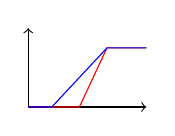
\begin{tikzpicture}
                \draw[<->] (0,1) |- (1.5,0);
                \draw[red] (0,0) -- (.65,0) -- (1,.75) -- (1.5,.75);
                \draw[blue] (0,0) -- (.3,0) -- (1,.75) -- (1.5,.75);
            \end{tikzpicture}
        \end{minipage}
        \begin{minipage}{0.5\textwidth}
            \begin{equation*}
                f_n(x) = \left\{\begin{array}{ll}
                    0 & \forall x \leq 1 - \frac{1}{n}\\
                    1 & \forall x > 1\\
                    \end{array}\right.
            \end{equation*}
        \end{minipage}
    \end{center}
    Donc $(f_n)_{n=1}^\infty$ est une suite de Cauchy car $||f_n - f_m||_2 \underset{m,n\to\infty}{\longrightarrow} 0$, mais ne converge vers rien car convergerait de manière discontinue :
    \begin{center}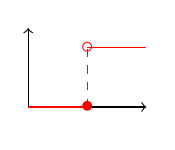
\begin{tikzpicture}
        \draw[<->] (0,1) |- (1.5,0);
        \draw[red] (0,0) -- (.75,0) node[] {\small{$\bullet$}};
        \draw[red] (.75,.75) node[]{\small{$\circ$}} -- (1.5,.75);
        \draw[red,dashed] (.75,0) -- (.75,.75);
    \end{tikzpicture}\end{center}
    Pour qu'effectivement, il existe une fonction $f$ respectant la relation ci-dessus, il faut que $f(x) = 0$ si $x<1$, 1 si $x>1$ et que $f\in C(I)$, ce qui est impossible. On conclut que l'espace des fonctions est donc incomplet.
\end{proof}

Pour espérer pouvoir rendre cet espace complet, on ne peut ni modifier la norme, ni le produit scalaire. On va alors ajouter une (ou plusieurs) propriété(s) (on va élargir l'espace) :
\begin{description}
    \item[Essai 1] $\mathcal{R}(I) = \{ f:I\to\mathbb{R} | f \ \mathrm{int\Acute{e}grable\ au\ sens\ de\ Riemannn,\ avec}\ \langle\cdot,\cdot\rangle \mathrm{ci-dessus} \} \ \cdots$ ECHEC :
        \begin{itemize}
            \item \textbf{Soucis 1 :} La norme induite $||f||_2$ est une semi-norme (pas une norme)
            \item \textbf{Soucis 2 :} $R(I)$ n'est pas complet...
        \end{itemize}
    \item[Essai 2] $C(I)\cup\{ (f_n)_{n=1}^\infty \big| (f_n)_{n=1}^\infty \subset C(I),\ \mathrm{sont\ de\ Cauchy\ et\ divergent\ pour}\ ||\cdot||_2\}$ (divergent signifie qu'il n'existe pas de fonction dans $C(I)$ qui soit de Cauchy). Le problème de cette propriété est que la fonction $||\cdot||$ serait alors une semi-norme.
    \item[Essai 3] $\mathcal{L}^2(I) = C(I)\cup\big\{ \{ (\Tilde{f}_n)_{n=1}^\infty\subset C(I)\big| ||\Tilde{f}_n-f_n||_2\to0 \}\bigg| (f_n)_{n=1}^\infty\subset C(I),\ \mathrm{Cauchy\ et\ divergente\ pour}\ ||\cdot||_2 \big\}$. Cet espace défini comme étant \textbf{la complétion} de $C(I)$ pour $||\cdot||_2$. On gardera cette définition là, malgré le fait qu'elle soit pas très pratique.
\end{description}


\subsection{Notion de convergence}

\begin{definition}
    Soit $X$ un espace muni d'une distance $d$ sur lequel est défini une suite de fonctions $(f_n)$ à valeurs réelles ou complexes. Si $\forall \epsilon > 0,\ \exists N\in\mathbb{N}$ tel que $\forall n\geq N,\ d(f_n,f)<\epsilon$, alors $f_n$ converge vers $f$ pour $n$ tendant vers l'infini.
\end{definition}

\begin{definition}
    Soit $X$ un espace vectoriel muni d'une norme $||\cdot||$ sur lequel est défini une suite de fonctions $(f_n)$ à valeurs réelles ou complexes. Si $\forall \epsilon > 0,\ \exists N\in\mathbb{N}$ tel que $\forall n\geq N,\ ||f_n - f||<\epsilon$, alors $f_n$ converge vers $f$ pour $n$ tendant vers l'infini.
\end{definition}

\begin{definition}
    Soit $X$ un espace vectoriel muni d'un produit scalaire $\langle\cdot,\cdot\rangle$ ($||\cdot|| = \sqrt{\langle\cdot,\cdot\rangle}$) sur lequel est défini une suite de fonctions $(f_n)$ à valeurs réelles ou complexes. Si $\forall \epsilon > 0,\ \exists N\in\mathbb{N}$ tel que $\forall n\geq N,\ \langle f_n,f \rangle <\epsilon$, alors $f_n$ converge vers $f$ pour $n$ tendant vers l'infini.
\end{definition}

\begin{definition}
    Soit $X$ un espace vectoriel muni d'une topologie $\mathcal{O}$ sur lequel est défini une suite de fonctions $(f_n)$ à valeurs réelles ou complexes. Cette suite de fonctions converge vers $f$ pour $n$ tendant vers l'infini f si $\forall \ \text{ouvert}\ O \ni f,\ \exists N\in\mathbb{N}$ tel que $\forall n\geq N,\ f_n \in O$.
\end{definition}


\subsection{Opérateurs linéaires}
% Section 2.3

\begin{definition}
    La relation linéaire $A$ entre les deux espaces normés $X$ et $Y$ est appelé \textbf{opérateur linéaire}
    \begin{equation*}
        A:\mathcal{D}(A)\subseteq X\rightarrow Y \qquad X,Y\ \mathrm{des\ espaces\ vectoriels}\ ||\cdot||^2.
    \end{equation*}
    si $\forall x_0,x_1 \in \mathcal{D}(A), \lambda_0,\lambda_1 \in \mathbb{C}$ : $\lambda_0x_0 + \lambda_1x_1 \in \mathcal{D}(A)$ et $A(\lambda_0x_0 + \lambda_1x_1) = \lambda_0A(x_0) + \lambda_1A(x_1)$.\\
    
    Le sous-espace linéaire $\mathcal{D}(A)$ sur lequel $A$ est défini est appelé \textbf{domaine} de $A$ et requiert fréquemment d'être dense. Le \textbf{noyau} (ou <<\textbf{null space}>>)
    \begin{equation*}
        \mathrm{Ker}(A) := \left\{ f\in\mathcal{D}(A)|Af = 0 \right\} \subseteq X \qquad (\text{= sous-espace vectoriel fermé})
    \end{equation*}
    et l'espace colonne
    \begin{equation*}
        \mathrm{Ran}(A) := \left\{ Af|f\in\mathcal{D}(A) \right\} = A\mathcal{D}(A) \subseteq Y
    \end{equation*}
    sont définis comme d'habitude.
\end{definition}

\begin{definition}
    L'opérateur $A$ est \textbf{borné} si
    \begin{equation*}
        ||A|| := \sup_{\scriptsize{\begin{array}{c}f\in\mathcal{D}(A) \\ ||f||_X=1\end{array}}} ||Af||_Y = \sup_{\scriptsize{\begin{array}{c}f\in\mathcal{D}(A) \\ ||f||_X\neq0\end{array}}} \frac{||Af||_Y}{||f||_X} < \infty.
    \end{equation*}
\end{definition}

\begin{theo}
    Un opérateur linéaire $A$ est borné si et seulement s'il est continu.
\end{theo}
\begin{proof}
    \begin{description}
        \item[borné $\Rightarrow$ continu] Borné $\Rightarrow\ ||Af||_Y \leq ||A||\ ||f||_X$ pour tout $f\in\mathcal{D}(A)$. On a donc que $A$ est de Lipschitz de constante $||A||$, et donc que $A$ est continu.
        \item[continu $\Rightarrow$ borné] Supposons que $A$ est continu et non borné. Alors il existe une suite $(u_n)_{n=1}^\infty$ de vecteur unitaire ($||u_n||_X=1$) telle que $||Au_n||_Y\geq n$. Alors $f_n := \frac{1}{n}u_n$ converge vers 0 mais pas $Af_n$ puisque $||Af_n||_Y \geq 1$. Si $A$ n'est pas borné, il n'est pas continu. On conclut donc que si $A$ est continu, alors il est borné.
    \end{description}
\end{proof}

\begin{theo}
    Soit $A:\mathcal{D}(A) \subset X \rightarrow Y $ un opérateur linéaire. Toutes les propriétés suivantes sont équivalentes :
    \begin{itemize}
        \item $A$ est borné
        \item l'image de $\mathcal{D}(A) \cap \overline{B_1}(0)$ est bornée
        \item l'image de tout sous-ensemble borné de $\mathcal{D}(A)$ est bornée
        \item $A$ est continu en $0$
        \item $A$ est continu sur $\mathcal{D}(A)$
        \item $A$ est Lipschitzien ($||Af-Ag||_Y \leq k ||f-g||_X \ \forall f,g \in \mathcal{D}(A),k\geq0$).
    \end{itemize}
\end{theo}

\begin{theo}
    Si $X$ est de dimension finie, alors tout opérateur est borné (et donc continu).
\end{theo}

\begin{proof}
    Soit $\{x_j\}_{j=1}^n$ une base de $X$. Tout vecteur $x \in X$ peut dès lors s'écrire $x=\sum \limits_{j=1}^n \alpha_jx_j$. Prenons sans pertes de généralité que $||x||_X = \sqrt{\sum \limits_{j=1}^n |a_j|^2}$ (dans un espace de dimension finie, toutes les normes sont équivalentes). Alors,
    \begin{equation*}
        ||Ax||_Y = ||A\sum \limits_{j=1}^n \alpha_jx_j||_Y \leq \sum_{j=1}^n |\alpha_j|||Ax_j||_Y \leq \sqrt{ \sum_{j=1}^n ||Ax_j||_Y^2}||x||_X
    \end{equation*}
    Donc $||A|| \leq \sqrt{\sum \limits_{j=1}^n ||Ax_j||_Y^2}$
\end{proof}

\begin{example}
    Soit $X=l^p(\mathbb{N})$ et $a\in l^\infty(\mathbb{N})$. Considérons l'opérateur multiplication $A:X\rightarrow Y$ défini par
    \begin{equation*}
        (Ab)_j := a_jb_j \ \forall b \in X.
    \end{equation*}
    Alors, $|(Ab)_j| \leq ||a||_\infty |b_j|$ montre que $||A||\leq||a||_\infty$. En réalité, on a même que $||A||=||a||_\infty$
\end{example}

\begin{example}
    Pour $X=l^p(\mathbb{N})$, on définit $A:X\rightarrow Y$ pour $f \in X$ par $(Af)_j = f_{j+1}$. Dès lors, on peut prouver que $||A|| = 1$. Le même résltat est obtenu pour l'application définie par $(Af)_1 = 0$ et $(Af)_j = f_{j-1}$.
\end{example}

\begin{example}
    Considérons l'espace vectoriel des fonctions différentiables $X=C^1[0,1]$ et équipons-le d'une norme
    \begin{equation*}
        ||f||_{\infty,1} := \max_{x\in[0,1]}|f(x)| + \max_{x\in[0,1]}|f'(x)|.
    \end{equation*}
    Soit $Y=C[0,1]$ muni de la norme $||\cdot||_\infty$. Nous observons que l'opérateur différentiel $A = \frac{d}{dx} : X\rightarrow Y$ (Soit $f \in C^1[0,1]$, $Af = f'\in C[0,1]$) est borné car
    \begin{equation*}
        ||Af||_Y = \max_{x\in[0,1]} |f'(x)| \leq \max_{x\in[0,1]} |f(x)| + \max_{x\in[0,1]} |f'(x)| = ||f||_{\infty,1} = ||f||_X.
    \end{equation*}
    Cependant, si nous considérons que $A=\frac{d}{dx}:\mathcal{D}(A)\subseteq Y\rightarrow Y$ défini sur $\mathcal{D}(A) = C^1[0,1]$, alors nous avons un opérateur non borné. Pour le montrer, choisissons
    \begin{equation*}
        u_n = \sin(n\pi x)
    \end{equation*}
    qui est normalisé par $||u_n||_\infty = 1$ et observons que
    \begin{equation*}
        Au_n(x) = u'_n(x) = n\pi\cos(n\pi x)
    \end{equation*}
    est non borné, $||Au_n||_\infty = n\pi$.
\end{example}

\begin{example}
    Soit $X=C[0,1]$. On définit $A:X \rightarrow X$ par $(Af)(x)=\int_0^xf(t)\ dt$. L'opérateur $A$ est borné et $||A||=1$ : $|\int_0^x f(t)\ dt| \leq x||f||_\infty$ et $||Af||_X = ||\int_0^x f(t)\ dt||_X$.
\end{example}

\begin{remark}
    Lorsqu'on prend la même norme dans les espaces de départ et d'arrivée, l'opérateur de dérivation n'est pas borné alors que celui d'intégration l'est! Cela provient du fait que l'intégration a une propriété de positivité de l'intégrale d'un fonction positive que la dérivée n'a pas.
\end{remark}

\begin{theo}
    Soit $A:\mathcal{D}(A)\subset X\to Y$ un opérateur linéaire et borné. Si $\mathcal{D}(A)$ est dense dans $X$ et que $Y$ est un espace de Banach (normé complet), il existe alors une seule extension continue $\overline{A}:\overline{\mathcal{D}(A)} \subset X \rightarrow Y$ linéaire et bornée telle que $||\overline{A}|| = ||A||$ et $\overline{A}\big|_{\mathcal{D}(A)} = A$ ($\overline{A}\big|_{\mathcal{D}(A)}$ = $\overline{A}$ restreint au domaine $\mathcal{D}(A)$).
\end{theo}
\begin{proof}
    \begin{description}
        \item[\textbf{Définition de $\overline{A}$ :}] Nous recherchons $\overline{A}f$ tel que $(f_n)_{n=1}^\infty\subset\mathcal{D}(A) \to f \in \overline{\mathcal{D}(A)}$ qui existe car $\mathcal{D}(A)$ est dense dans $X$. Comme $Y$ est complet, on peut poser $\overline{A}f = \lim_{n\to\infty}Af_n$, qui existe car $(f_n)$ converge et est donc une suite de Cauchy, donc $(Af_n)$ est également de Cauchy et converge.
        
        Montrons que $\overline{A}f$ est indépendant de la suite $f_n$ choisie : soit $(g_n)\subset\mathcal{D}(A)$ tel que $g_n \to f$. On a
        \begin{align*}
            ||Af_n - Ag_n||_Y & = ||A(f_n - g_n)||_Y \\
            & \leq ||A||\ ||f_n - g_n||_X \to 0 \\
            \Rightarrow \lim \limits_{n\to \infty}||\overline{A}f - Ag_n||_Y & = \lim \limits_{n\to \infty}||Af_n - Ag_n||_Y = 0.
        \end{align*}
        On conclut alors que $Ag_n\to\overline{A}f$.
        \item[\textbf{Restriction :}] $\overline{A}$ est bien une extension de $A$ car si on choisit $f \in \mathcal{D}(A)$ tel que $f_n = f$, on a $\overline{A}f = \lim \limits_{n \to\infty} Af = Af$.
        \item[\textbf{$\overline{A}$ est linéaire :}]
        \begin{align*}
            \overline{A}(\alpha f + \beta g) & = \lim_{n\to\infty} A(\alpha f_n + \beta g_n) \\ & = \lim_{n\to\infty} (\alpha A f_n + \beta A g_n) \\
            & = \alpha\overline{A} f + \beta\overline{A} g.
        \end{align*}
        \item[\textbf{Borne :}] Montrons que $||\overline{A}|| = ||A||$ :
        \begin{align*}
            ||\overline{A}|| & = \sup_{||f||_X=1} ||\overline{A}f||_Y \\ & = \sup_{||f||_X=1} ||\lim_{n\to\infty}Af_n||_Y \\
            & = \sup_{||f||_X=1} \lim_{n\to\infty}||Af_n||_Y \\ & \leq \sup_{||f||_X=1} \lim_{n\to\infty}||A||\ ||f_n||_X \\
            & = \sup_{||f||_X=1}||A|| \underbrace{\lim_{n\to\infty} ||f_n||_X}_{||f||_X} \\
            & = ||A||
        \end{align*}
    \end{description}
\end{proof}

\begin{definition}
    On représente par $\mathcal{L}(X,Y)$ l'ensemble des opérateurs linéaires bornés de $X$ dans $Y$ : $\mathcal{L}(X,Y) = \{A:X \to Y | A$ est linéaire et bornée$\}$ . On admet les deux énoncés suivant :
    \begin{itemize}
        \item $\mathcal{L}(X) := \mathcal{L}(X,X)$ et
        \item $X^\star := \mathcal{L}(X,\mathbb{C})$ est l'ensemble \textbf{dual} de $X$. Les éléments de $X^\star$ sont appelés \textbf{fonctionnelles linéaires bornés}.
    \end{itemize}
\end{definition}

\begin{example}
    Soit l'espace $X=l^p(\mathbb{N})$. On définit $l_j(a) := a_j$. On a alors $l_j\in X^\star$. On cherche alors $||l_j||$.
    \begin{equation*}
        \left.\begin{array}{rcl}
            |l_j(a)| = |a_j| \leq \big[\sum \limits_{j\in\mathbb{N}} |a_j|^p\big]^\frac{1}{p} = ||a||_p & \Rightarrow & ||l_j|| \leq 1 \\
            |l_j(\delta^j)| = 1 & \Rightarrow & ||l_j|| \geq 1
        \end{array}\right\} ||l_j|| = 1.
    \end{equation*}
\end{example}

\begin{example}
    Soit l'espace $X=C[0,1]$ avec la norme $||\cdot||_\infty$. Soit $f\in X$. On définit l'opérateur $l$ par $lf := f(1)$. Alors $l\in X^\star$ car $|lf|=|f(1)|\leq \sup \limits_{[0,1]}|f| = ||f||_\infty$. En fait, $||l|| = 1$.
    
    $l \not\in \mathcal{L}^2_{cont}[0,1]^\star$ : si $f_n(x) = \sqrt{n}x^{\frac{n-1}{2}}$, on a $||f_n||_2 = \sqrt{\int_0^1|f_n(x)|^2 \ dx} = \sqrt{\int_0^1 nx^{n-1} \ dx} = [x^n]_0^1=1$ mais $|lf_n| = \sqrt{n}\to \infty$.
\end{example}

\begin{theo}
    $\mathcal{L}(X,Y)$ avec la norme d'opérateur est un espace vectoriel normé, et de Banach si $Y$ est de Banach.
\end{theo}

\begin{example}
    $X = C[0,1],\ ||\cdot||_\infty$. Soit $g$ et $f_n$ intégrables sur $[0,1]$. On a
    \begin{equation*}
        l_g(f) := \int_0^1 g(x)f(x)\ dx.
    \end{equation*}
    Alors $l_g\in X^\star$ avec $||l_g|| = \int_0^1 |g(x)|dx =: ||g||_1$ :
    \begin{itemize}
        \item $|l_gf| = |\int_0^1 f(x)g(x) \ dx| \leq \int_0^1|f(x)|\ |g(x)| \ dx \leq ||f||_\infty \int_0^1|g(x)| \ dx \implies ||l_g||\leq\int_0^1|g(x)|\ dx$
        \item Soit $\epsilon>0$. On pose $f_\epsilon=\frac{g^*}{|g|+\epsilon}$ ($g^*$ = conjugué de g).Dès lors, $||f_\epsilon||_\infty = \sup\limits_{[0,1]} \frac{|g|}{|g|+\epsilon}\leq1$
        
        $||l_g|| \geq |l_gf_\epsilon| = \int_0^1\frac{|g(x)|^2}{|g(x)|+\epsilon}\ dx \geq \int_0^1 \frac{|g(x)|^2-\epsilon^2}{|g(x)|+\epsilon}\ dx \geq \int_0^1 |g(x)|-\epsilon\ dx = \int_0^1 |g(x)| \ dx - \epsilon$.
    \end{itemize}
\end{example}



%partie 2 : voir syntheses prof
\section{Espaces de Hilbert}
\sectionmark{Espaces de Hilbert}


\subsection{Bases orthonormées}
% Sous-section 3.1

\begin{definition}
    Un ensemble $\{u_j\}_{j\in\mathcal{J}}\subset\mathcal{H}$ est un ensemble orthonormé si $\langle u_j,u_k \rangle = \delta_{jk}$. L'ensemble d'indice $\mathcal{J}$ peut être un ensemble fini ou non, dénombrable ou non.
    
    Un ensemble orthonormé est formé de vecteurs linéairments indépendants.
\end{definition}
\begin{proof}
    Considérons un vecteur $a = \sum \limits_{l=1}^m \alpha_lu_{j_l} = 0$. Le produit scalaire de $a$ avec $u_{j_n}$ donne : $\langle a,u_{j_n} \rangle = \langle \sum \limits_{l=1}^m \alpha_lu_{j_l}, u_{j_n} \rangle = \sum \limits_{l=1}^m \alpha_l \langle u_{j_l},u_{j_n} \rangle = \alpha_n = 0$. Si nous effectuons cette opération pour différents $n$, nous observons que $a = 0$ ssi $\alpha_l = 0 \ \forall l$.
\end{proof}

\begin{lemme}
\label{lemme:Bessel}
    Soit $\{u_j\}_{j=1}^n$ un ensemble orthonormé fini et $f\in\mathcal{H}$. Alors
    \begin{equation*}
        \left\{ \begin{array}{rcll}
            f & = & f_\bot + f_\sslash  \\
            f_\sslash & = & \sum_{j} \alpha_j u_j & \mathrm{c\Grave{a}d}\ f_\sslash\in\setSpan\{u_j\}_{j=1}^n \\
            f_\bot & \bot & u_{j,\sslash} & \mathrm{c\Grave{a}d}\ \langle u_j,f_\bot \rangle = 0\ \forall j
        \end{array} \right.
    \end{equation*}
    a une et une seule solution donnée par
    \begin{equation*}
        f_\sslash = \sum_{j=1}^n \langle u_j,f \rangle u_j.
    \end{equation*}
    On a alors $||f||^2 = \sum_{j=1}^n \big|\langle u_j,f \rangle\big|^2 + ||f_\bot||^2$.
    
    $f_\sslash$ est la projection de $f$ sur $\setSpan\{ u_1,u_2,\cdots,u_n \}$. Soit $\hat{f}= \sum \limits_{j=1}^n\alpha_ju_j$. Dès lors,
    \begin{align*}
        ||f-\hat{f}||^2 &= ||f_\sslash + f_\bot -\hat{f}||^2 \\
        &= ||f_\bot||^2 + ||\sum \limits_{j=1}^n \big( \langle u_j,f\rangle - \alpha_j\big)u_j||^2\\
        &= ||f_\bot||^2 + \sum \limits_{j=1}^n|\langle u_j,f\rangle -\alpha_j|^2
    \end{align*}
    Donc, $||f-\hat{f}||^2 \geq ||f_\bot||^2$ et $||f-\hat{f}||^2$ est minimal pour $\alpha_j=\langle u_j,f \rangle$.
\end{lemme}

\begin{theo}[Inégalité de Bessel]
    \begin{equation*}
        ||f||^2 \geq \sum_{j=1}^n \big|\langle u_j,f \rangle\big|^2
    \end{equation*}
\end{theo}

On peut maintenant généraliser dans le cas où $\{u_j\}$ est de dimension infinie. Définissons tout d'abord la notion de \textbf{somme infinie}.

\begin{definition}
    Considérons une famille de nombres positifs $\{a_j\}_{j\in\mathcal{J}}$. La somme est définie par
    \begin{equation*}
        \sum_{j\in\mathcal{J}} a_j = \sup\left\{\sum_{j\in K} a_j\big| K\subseteq \mathcal{J} < \infty\right\}
    \end{equation*}
    Dès lors, on a $\sum_{j\in\mathcal{J}} a_j \geq \sum_{j\in K} a_j$.
\end{definition}

Soit $\{u_j\}_{j\in\mathcal{J}}$ un ensemble orthonormé dans $\mathcal{H}$, si $K\subseteq\mathcal{J}<\infty$, on a par l'inégalité de Bessel : 
\begin{equation*}
    \sum\limits_{j\in K}|\langle u_j,f\rangle|^2 \leq ||f||^2.
\end{equation*}
Dès lors, 
\begin{equation*}
    \sum\limits_{j\in \mathcal{J}}|\langle u_j,f\rangle|^2 = \sup\left\{\sum_{j\in K} |\langle u_j,f\rangle|^2 \big| K\subseteq \mathcal{J} < \infty\right\} \leq ||f||^2
\end{equation*}

Par définition de suprémum, $\exists (K_n)_{n\in\mathbb{N}}\subset \mathcal{J}$ tels que
\begin{equation*}
    \lim_{n\to\infty} \sum_{j\in K_n} |\langle u_j,f\rangle|^2 = \sum_{j\in\mathcal{J}} |\langle u_j,f\rangle|^2
\end{equation*}

Prenons maintenant, $K_m,K_n \subset \mathcal{J} < \infty$ et posons $f_n = \sum_{j\in K_n} \langle u_j,f\rangle u_j \in \mathcal{H}$.
\begin{align*}
    ||f_n-f_m||^2 & = ||\sum_{j\in K_n} \langle u_j,f\rangle u_j - \sum_{j\in K_m} \langle u_j,f\rangle u_j||^2\\
    & = \left\langle \sum_{j\in K_n} \langle u_j,f\rangle u_j - \sum_{j\in K_m} \langle u_j,f\rangle u_j , \sum_{j\in K_n} \langle u_j,f\rangle u_j - \sum_{j\in K_m} \langle u_j,f\rangle u_j\right\rangle\\
    & = \left\langle \sum_{j\in K_n} \langle u_j,f\rangle u_j,\sum_{j\in K_n} \langle u_j,f\rangle u_j\right\rangle + \left\langle \sum_{j\in K_m} \langle u_j,f\rangle u_j ,  \sum_{j\in K_m} \langle u_j,f\rangle u_j \right\rangle\\
    & - 2\left\langle \sum_{j\in K_n} \langle u_j,f\rangle u_j ,  \sum_{j\in K_m} \langle u_j,f\rangle u_j \right\rangle\\
    & = \Big[\sum_{j\in K_n} \langle u_j,f\rangle\Big]^2 \langle u_j,u_j\rangle + \Big[\sum_{j\in K_m} \langle u_j,f\rangle\Big]^2 \langle u_j,u_j\rangle - 2 \Big[\sum_{j\in K_n} \langle u_j,f\rangle\Big]^2 \langle u_j,u_j\rangle\\
    & = \sum_{j\in K_n} |\langle u_j,f\rangle|^2 + \sum_{j\in K_m} |\langle u_j,f\rangle|^2 - 2 \sum_{j\in (K_n \cap K_m)} |\langle u_j,f\rangle|^2\\
    & = -\sum_{j\in K_n} |\langle u_j,f\rangle|^2 - \sum_{j\in K_m} |\langle u_j,f\rangle|^2 + 2 \sum_{j\in (K_n \cup K_m)} |\langle u_j,f\rangle|^2\\
    & \leq  -\sum_{j\in K_n} |\langle u_j,f\rangle|^2 - \sum_{j\in K_m} |\langle u_j,f\rangle|^2 + 2 \sum_{j\in \mathcal{J}} |\langle u_j,f\rangle|^2
\end{align*}

En faisant tendre $n,m$ vers l'infini, on trouve que $||f_n-f_m||^2 \to 0$. De plus, si $\mathcal{H}$ est un ensemble complet, on sait que la suite $f_n$ converge vers $\sum \limits_{j\in\mathcal{J}} \langle u_j,f\rangle u_j$.

Considérons une autre suite $(\widetilde{K}_n)_{n\in\mathbb{N}}$ avec $\widetilde{f}_n = \sum_{j\in \widetilde{K}_n} \langle u_j,f\rangle u_j$. On trouve que $\sum_{j\in \mathcal{J}} \langle u_j,f\rangle u_j$ est indépendant du choix de la suite d'ensembles finis :
\begin{equation*}
    ||f_n - \widetilde{f}_n||^2 \leq  -\sum_{j\in K_n} |\langle u_j,f\rangle|^2 - \sum_{j\in \widetilde{K}_n} |\langle u_j,f\rangle|^2 + 2 \sum_{j\in \mathcal{J}} |\langle u_j,f\rangle|^2 \to 0
\end{equation*}

On peut maintenant généraliser le lemme \ref{lemme:Bessel} en dimension infinie : tout $f \in \mathcal{H}$ peut s'écrire sous la forme $f=f_\sslash + f_\bot$ avec $\langle f_\sslash,f_\bot \rangle = 0$ et $f_\sslash = \sum\limits_{j\in\mathcal{J}} \langle u_j,f\rangle u_j$. De plus, $\langle u_j,f_\bot\rangle = 0$ et $||f||^2 =\sum\limits_{j\in\mathcal{J}} |\langle u_j,f\rangle|^2+||f_\bot||^2$.

Ensuite, $\forall \hat{f} \in \overline{\text{span}(\{u_j\})}$ (adhérence des combilis de $\{u_j\}$), $||f-\hat{f}||^2\geq||f_\bot||^2$ avec égalité ssi $f_\sslash=\hat{f}$.

\begin{definition}
    Un ensemble orthonormé $\{u_j\}_{j\in\mathcal{J}}$ est une \textbf{base orthonormée} de l'espace $\mathcal{H}$ si $\forall f\in\mathcal{H}$
    \begin{equation*}
        f = \sum_{j\in\mathcal{J}} \langle u_j,f \rangle u_j
    \end{equation*}
\end{definition}

\begin{example}
    Les vecteur de la suite $(\delta^n_j)_{j\in\mathbb{N}}$ tels que $\delta^n_j=1$ ssi $n=j$ forment une base de $l^2(\mathbb{N})$
\end{example}
\begin{proof}
    Prenons un vecteur $a\in l^2(\mathbb{N})$. Dès lors, on a que $\sum \limits_{j=1}^n \langle \delta^j,a\rangle\delta^j$ donne les $n$ premières composantes du vecteur $a$. Donc, $||\sum \limits_{j=1}^n \langle \delta^j,a\rangle\delta^j-a||^2 = \sum \limits_{j=n+1}^\infty |a_j|^2$. Or on sait que $||a||_2$ est finie donc le dernier élément de $a$ tend vers $0$ ce qui permet de conclure : $||\sum \limits_{j=1}^n \langle \delta^j,a\rangle\delta^j-a||^2 \underset{n\to\infty}{\longrightarrow}0$.
\end{proof}

\begin{theo}[Gram-Schmidt]
    Tout espace de Hilbert séparable a une base orthonormée dénombrable.
\end{theo}
\begin{proof}
    Par définition de séparabilité, il existe un ensemble $\{f_n\}$ dénombrable et dense dans $\mathcal{H}$. On va procéder de manière récursive afin de trouver une base.
    
    Tout d'abord, retirons de l'ensemble $\{f_n\}$ les éléments $f_n$ qui sont une combinaison linéaire des éléments $f_1,...,f_{n-1}$. Ensuite, on pose $\widetilde{f}_n = f_n-\sum_{j=1}^{n-1}\langle u_j,f\rangle u_j \neq 0$ par indépendance linéaire. Le nouvel élément de la base doit être normalisé et vaut donc $u_n = \frac{\widetilde{f}_n}{||\widetilde{f}_n||}$.
    
    On a donc le procédé de Gram-Schmidt : $\{u_j\}_{j=1}^\infty$ défini récursivement par
    \begin{equation*}
        u_n = \frac{f_n - \sum_{j=1}^{n-1} \langle u_j,f \rangle u_j}{\left|\left|f_n - \sum_{j=1}^{n-1} \langle u_j,f \rangle u_j \right|\right|}
    \end{equation*}
    
    Si $\text{dim}\mathcal{H}<\infty$, $\{f_n\}$ est un ensemble fini et $\{u_n\}$ est une base au sens algébrique.
\end{proof}

\begin{example}
    Considèrons $\mathcal{L}^2_{cont}[-1,1]$ muni du produit scalaire $\langle f,g \rangle = \int_{-1}^1 f^*(x)g(x) \ dx$. Étant donné que les polynômes sont denses dans cet ensemble, on peut trouver une base orthonormée en partant de $f_n(x)=x^n$ pour $n\in\mathbb{N}$ :
    \begin{table}[H]
        \centering
        \begin{tabular}{ll}
            $\widetilde{f}_0(x) = 1$ & $u_0(x)=\frac{1}{\sqrt{\int_{-1}^1 1 \ dx}} = \sqrt{\frac{1}{2}}$ \\
            $\widetilde{f}_1(x) = x-\frac{1}{\sqrt{2}}\int_{-1}^1 \frac{x}{\sqrt{2}} \ dx = x$ & $u_1(x)=\frac{x}{\sqrt{\int_{-1}^1 x^2 \ dx}} = \sqrt{\frac{3}{2}}x$ \\
            $\widetilde{f}_2(x) = x^2-\frac{1}{\sqrt{2}}\int_{-1}^1 \frac{x^2}{\sqrt{2}} \ dx - \sqrt{\frac{3}{2}}x\int_{-1}^1 \sqrt{\frac{3}{2}}x^3 \ dx = x^2 - \frac{1}{3}$ & $u_2(x)=\frac{x^2 - \frac{1}{3}}{\sqrt{\int_{-1}^1 \big(x^2 - \frac{1}{3}\big)^2 \ dx}} = \sqrt{\frac{5}{2}}\frac{3x^2-1}{2}$ \\
        \end{tabular}
    \end{table}
    Les polynômes obtenus sont appelés les polynômes de Legendre.
\end{example}

\begin{theo}
    Pour un ensemble orthonormé $\{ u_j \}_{j\in\mathcal{J}}$ de $\mathcal{H}$, les conditions suivantes sont équivalentes :
    \begin{enumerate}[label=(\roman*)]
        \item $\{ u_j \}_{j\in\mathcal{J}}$ forment un ensemble orthormé maximal (on ne peut pas ajouter un vecteur à l'ensemble tout en gardant un ensemble orthonormé);
        \item $\{ u_j \}_{j\in\mathcal{J}}$ forment une base orthonormée, c'est-à-dire que pour tout $f\in\mathcal{H}$, $f = \sum_{j\in\mathcal{J}} \langle u_j,f \rangle u_j$
        \item $\forall f\in\mathcal{H}$ : $||f||^2 = \sum_{j\in\mathcal{J}} \big| \langle u_j,f \rangle \big|^2$ (relation de Parseval) ;
        \item $\{f\in\mathcal{H}\big|\forall j\in\mathcal{J}, \ \langle u_j,f \rangle = 0\} = \{0\}$.
    \end{enumerate} \label{theo:ens_ortho}
\end{theo}
\begin{proof}
    Puisque les éléments de $\{ u_j \}_{j\in\mathcal{J}}$ sont orthormaux entre eux, on a pour tout $f\in\mathcal{H}$ que
    \begin{enumerate}[label=(\alph*)]
        \item $f = \sum_{j\in\mathcal{J}} \langle u_j,f \rangle u_j + f_\bot$ où $f_\bot$ est perpendiculaire à $u_j$ pour tout $j$ ;
        \item $||f||^2 = \sum_{j\in\mathcal{J}} \big|\langle u_j,f \rangle\big|^2 + ||f_\bot||^2$
        \item $||f-f_\sslash|| \leq \left|\left| f - \sum_{j\in\mathcal{J}}\alpha_j u_j \right|\right|$ pour tout $\alpha_j\in\mathbb{R}$.
    \end{enumerate}
    \begin{description}
        \item[\textit{(i)$\Rightarrow$(ii)}] Si non-\textit{(ii)}, il existe un vecteur perpendiculaire à tous les autres, notamment $f_\bot = f-\sum_{j\in\mathcal{J}}\langle u_j, f\rangle u_j \neq 0$, qu'on peut normaliser et ajouter à la base et $\{u_j\}_{j\in\mathcal{J}} \cup \{\frac{f_\bot}{||f_\bot||}\ $ serait un ensemble orthonormé (non-\textit{(i)}).
        \item[\textit{(ii)$\Rightarrow$(iii)}] Si \textit{(ii)}, alors $f_\bot = 0$ dans (a), de même que dans (b), donc \textit{(iii)}.
        \item[\textit{(iii)$\Rightarrow$(iv)}] Si \textit{(iii)} et $\langle u_j,f \rangle = 0$ $\forall j\in\mathcal{J}$, alors $||f||^2 = 0$, donc $f=0$.
        \item[\textit{(iv)$\Rightarrow$(i)}] Si non-\textit{(i)}, donc si $\{u_j\}$ n'est pas maximal, on peut trouver $\{u_j\}\cup\{g\}$ qui serait orthonormé. Or $g\in \mathcal{H}$ et donc des hypothèses de \textit{(iv)} on en conclut que $\langle u_j,g\rangle = 0 \implies g = 0$.
    \end{description}
\end{proof}

\iffalse
\begin{definition}
    Un opérateur $U\in\mathcal{L(\mathcal{H}_1,\mathcal{H}_2)}$ est \textbf{unitaire} s'il est bijectif et que
    \begin{equation}
        \langle U_g,U_f \rangle_2 = \langle g,f \rangle_1 \quad \forall g,f \in \mathcal{H}_1.
    \end{equation}
    Dans ce cas, on dit que $\mathcal{H}_1$ et $\mathcal{H}_2$ sont \textbf{unitairement équivalents}.
\end{definition}

\begin{theo}
    Tout espace de Hilbert séparable de dimension infinie est unitairement équivalent à $l^2(\mathbb{N})$.
\end{theo}
\begin{proof}
    Soit $\{u_j\}_{j\in\mathbb{N}}$ une base orthormale de $\mathcal{H}$. Montrons que $U:\mathcal{H}\to l^2(\mathbb{N}) : f\mapsto(\langle u_j,f \rangle)_{j\in\mathbb{N}}$ est unitaire.
    \begin{itemize}
        \item[$\bullet$] Il préserve la norme au vu du théorème \ref{theo:ens_ortho} ;
        \item[$\bullet$] Il est injectif
        \item[$\bullet$] Il est surjectif car pour tout $a\in l^2(\mathbb{N})$, $f:=\sum_{j\in\mathbb{N}} a_j u_j$ est bien défini et $U_f=a$.
    \end{itemize}
\end{proof}

\begin{theo}
    Tout espace de Hilbert admet une base orthonormale.
\end{theo}

\fi

\subsection{Projection de Riesz}
% Sous-section 3.2
\begin{theo}[Projection]
    Si $M \subset \mathcal{H}$ est un sous espace vectoriel fermé de $\mathcal{H}$, il existe un opérateur $P_M \in \mathcal{L}(\mathcal{H},\mathcal{H})$ tel que $\forall f\in\mathcal{H}$, $P_Mf \in M$ et $\forall f \in \mathcal{H},g\in M$, $\langle f-P_Mf,g\rangle=0$.
    
    En particulier, $\forall g\in M$, $||P_Mf-f||\leq||g-f||$ et $\forall f \in M$, $P_Mf = f$.
\end{theo}
\begin{proof}
    Comme $M$ est un sous-espace FERMÉ de Hilbert, il est lui même un espace de Hilbert. Posons $P_Mf = \sum_{j\in\mathcal{J}} \langle u_j,f\rangle u_j$ où $\{u_j\}$ est une base orthonormée de $M$ (l'opérateur $P_M$ renvoie $f_\sslash$). L'espace $M$ doit être fermé car $M=\{f\in\mathcal{H}\big|f=P_Mf\}$.
    
    Si on pose $M^\bot = \{f\big|\langle g,f\rangle=0 \ \forall g\in M\}$, on obtient $P_{M^\bot}f=f - P_Mf \implies P_{M^\bot} + P_M = I$
    
    $P_M$ est appelé \textbf{projection orthogonal} de $M$. 
\end{proof}

\begin{lemme}[Riesz]
    Si $\mathcal{H}$ est un espace de Hilbert, alors, pour toute fonctionnelle linéaire $l\in\mathcal{H}^\star=\mathcal{L}(\mathcal{H},\mathbb{C})$, il existe un vecteur $g\in\mathcal{H}$ tel que $\forall f\in\mathcal{H}$, on ait $l(f)=\langle f,g\rangle$.
\end{lemme}
\begin{proof}
    \begin{itemize}
        \item Si $l=0$, $l(f)=0 \ \forall f \in \mathcal{H}$ et $g=0$;
        \item Sinon, on a $\text{Ker}(l)=\{f\big|l(f)=0\}\subset \mathcal{H}$. On prend alors $\widetilde{g}\in\text{Ker}(l)^\bot$ tel que $||\widetilde{g}||=1$. On pose $g = l(\widetilde{g})^*\widetilde{g}$. Dès lors, $ \forall f\in\mathcal{H}$,
        \begin{equation*}
            l(f) = l(\widetilde{g})\langle \widetilde{g},f\rangle+\langle\widetilde{g},l(f)\widetilde{g}-l(\widetilde{g})f\rangle = l(\widetilde{g})\langle\widetilde{g},f\rangle=\langle g,f\rangle
        \end{equation*}
        car $l(l(f)\widetilde{g}-l(\widetilde{g})f)=l(f)l(\widetilde{g})-l(\widetilde{g})l(f)=0$.
    \end{itemize}
\end{proof}

\subsection{Séries de Fourier}
% Sous-section 3.3

\begin{definition}
    Soit $f:[-\pi,\pi]\to\mathbb{C}$ une fonction intégrable. Sa \textbf{série de Fourier} s'écrit
    \begin{equation*}
        S(f)(x) = \frac{a_0}{2} + \sum_{k\in\mathbb{N}}[a_k\cos(kx)+b_k\sin(kx)] = \sum_{k\in\mathbb{Z}}\hat{f}_ke^{ikx}
    \end{equation*}
    avec les coeeficients de Fouriers suivants
    \begin{align*}
        a_k & = \frac{1}{\pi}\int_{-\pi}^\pi \cos(kx)f(x) \ dx\\
        b_k & = \frac{1}{\pi}\int_{-\pi}^\pi \sin(kx)f(x) \ dx\\
        \hat{f}_k & = \frac{1}{2\pi}\int_{-\pi}^\pi e^{-iky}f(y) \ dy
    \end{align*}
\end{definition}

\begin{definition}
    Cette série peut s'écrire à l'aide du \textbf{noyau de Dirichlet} :
    \begin{equation*}
        S_n(f)(x) = \sum_{k=-n}^n\hat{f}_ke^{ikx} = \frac{1}{2\pi}\int_{-\pi}^\pi D_n(x-y)f(y)dy
    \end{equation*}
    avec
    \begin{equation*}
        D_n(x) = \sum_{k=-n}^n e^{ikx} = \frac{e^{i(n+1)x}-e^{-inx}}{e^{ix}-1} = \frac{e^{i(n+\frac{1}{2})x}-e^{-i(n+\frac{1}{2})x}}{e^{\frac{ix}{2}}-e^{\frac{-ix}{2}}} = \frac{\sin[(n+\frac{1}{2})x]}{\sin[\frac{x}{2}]}
    \end{equation*}
    Cette fonction satisfait les propriétés suivantes :
    \begin{itemize}
        \item $D_n(-x)=D_n(x)=D_n(x+2\pi)$
        \item $|D_n(x)|_{max} = D_n(0)=2n+1$
        \item $\int_{-\pi}^\pi D_n(x)\ dx = \sum\limits_{k=-n}^n \int_{-\pi}^\pi e^{ikx}\ dx = \sum_{k=-n}^n \frac{2\sin(k\pi)}{k} = 2\pi$ (tout s'annule sauf en $k=0$ où on obtient $\frac{0}{0}$ et en faisant l'hospital on obtient $\frac{2\pi\cos(k\pi)}{1}=2\pi$)
    \end{itemize}
\end{definition}

\begin{theo}
    Si on muni $ L^2[-\pi,\pi]$ (espace de Lebesgue :  fonctions telles que $f^p$ est intégrable au sens de Lebesgue) du produit scalire $\langle f,g\rangle = \frac{1}{2\pi}\int_{-\pi}^\pi f^*g$, les fonctions $\{e^{ikx}\}_{k\in\mathbb{N}}$ forment un ensemble orhtonormé. En effet,
    \begin{equation*}
        \int_{-\pi}^\pi e^{-ikx}e^{ilx} \ dx = \int_{-\pi}^\pi e^{ix (l-k)} \ dx = \Bigg[\frac{e^{ix(l-k)}}{i(l-k)}\Bigg]_{-\pi}^\pi = 2\pi\delta_{l,k}
    \end{equation*}
    donc $\langle e^{ikx},e^{ilx}\rangle = \delta_{k,l}$.
    
    De plus, cet ensemble est une base de $ L^2[-\pi,\pi]$ donc :
    \begin{itemize}
        \item $\{e^{ikx}\}_{k\in\mathbb{Z}}$ est un ensemble orthonormé maximal de $ L^2[-\pi,\pi]$
        \item $\forall f\in L^2[-\pi,\pi],\ \lim\limits_{n\to\infty}||S_n(f)-f||=0$ (convergence ponctuelle)
        \item $\forall f\in L^2[-\pi,\pi],\ \sum\limits_{k\in\mathbb{Z}}|\hat{f}_k|^2=\frac{1}{2\pi}\int_{-\pi}^\pi |f(x)|^2\ dx$
        \item si $f\in L^2[-\pi,\pi]$ et $\int_{-\pi}^\pi e^{ikx}f(x)\ dx = 0$ pour tout $k\in\mathbb{N}$, alors $f=0$.
    \end{itemize}
\end{theo}

Mais si $f$ est une fonction continue, la suite $(S_nf)$ ne converge pas toujours vers $f$ (de manière uniforme)... On va donc s'intéresser à la moyenne de la série de Fourier.

\begin{definition}
    On définit les \textbf{sommes de Fourier moyennées} par
    \begin{equation*}
        \overline{S}_n(f)(x)=\frac{1}{n}\sum_{k=0}^{n-1}S_k(f) = \frac{1}{2\pi}\int_{-\pi}^\pi F_n(x-y)f(y)\ dy
    \end{equation*}
    où $F_n$ est le \textbf{noyau de Fejér} :
    \begin{align*}
        F_n(x) &= \frac{1}{n} \sum_{k=0}^{n-1}D_k(x)
        = \frac{1}{2in\sin\big(\frac{x}{2}\big)}\sum_{k=0}^{n-1}e^{i(k+\frac{1}{2})x}-e^{-i(k+\frac{1}{2})x}\\
        & = \frac{1}{2in\sin\big(\frac{x}{2}\big)} \Bigg(\frac{e^{i(n+\frac{1}{2})x}-e^{\frac{ix}{2}}}{e^{ix}-1}-\frac{e^{-i(n+\frac{1}{2})x}-e^{\frac{ix}{2}}}{e^{-ix}-1}\Bigg)\\
        & = \frac{e^{inx}-2+e^{-inx}}{2in\sin\big(\frac{x}{2}\big)(e^{\frac{ix}{2}}-e^{\frac{-ix}{2}}} = \frac{\big(e^{\frac{inx}{2}}-e^{\frac{-inx}{2}}\big)^2}{2in\sin\big(\frac{x}{2}\big)(e^{\frac{ix}{2}}-e^{\frac{-ix}{2}}}
        = \frac{1}{n}\Bigg(\frac{\sin\big(\frac{nx}{2}\big)}{\sin\big(\frac{x}{2}\big)}\Bigg)^2
    \end{align*}
    Cette fonction satisfait les propriétés suivantes :
    \begin{itemize}
        \item $F_n(-x)=F_n(x)=F_n(x+2\pi)\geq0$
        \item $\int_{-\pi}^\pi F_n(x)\ dx = 2\pi$
    \end{itemize}
\end{definition}

\begin{theo}[Fejer]
    Soit $f:\mathbb{R}\to\mathbb{C}$ une fonction continue et périodique de période $2\pi$, alors $\overline{S}_n(f)\to f$ uniformément.
\end{theo}
\begin{proof}
    Par périodicité de $F_n$ et $f$ :
    \begin{equation*}
        \overline{S}_n(f)(x) = \frac{1}{2\pi}\int_{-\pi}^\pi F_n(x-y)f(y)\ dy = \frac{1}{2\pi}\int_{-\pi}^\pi F_n(z)f(x-z)\ dz
    \end{equation*}
    \begin{equation*}
        \overline{S}_n(f)(x)-f(x) = \frac{1}{2\pi}\int_{-\pi}^\pi F_n(z)[f(x-z)-f(x)]\ dz
    \end{equation*}
    On peut en déduire que $\forall \delta>0$ :
    \begin{align*}
        |\overline{S}_n(f)(x)-f(x)| & = \frac{1}{2\pi}\int_{-\pi}^\pi F_n(z)|f(x-z)-f(x)|\ dz\\
        & = \frac{1}{2\pi}\Bigg(\int_{-\delta}^\delta F_n(z)|f(x-z)-f(x)|\ dz + \int_{-\pi}^{-\delta} F_n(z)|f(x-z)-f(x)|\ dz \\
        & + \int_{\delta}^\pi F_n(z)|f(x-z)-f(x)|\ dz\Bigg)\\
        & \leq \sup\limits_{z\in[-\delta,\delta]}|f(x-z)-f(x)|+\frac{2||f||_\infty}{n\sin\big(\frac{\delta}{2}\big)^2}
    \end{align*}
    car $\int_{-\delta}^\delta F_n(z)\ dz\leq 2\pi$, $F_n(x)\leq\frac{1}{n\sin\big(\frac{\delta}{2}\big)^2}\ \forall \delta\leq|x|\leq\pi$ et $|f(x-z)-f(x)| \leq 2||f||_\infty$ (et $\pi-\delta\leq\pi$).
    
    Comme $f$ est uniformément continue, si on prend $\delta$ suffisamment petit, le premier terme va valoir $0$. On choisit ensuite $n$ suffisamment grand afin de rendre le second terme faible. On trouve donc que $\overline{S}_n(f)$ converge uniformément vers $f$.
\end{proof}

On peut utiliser ce résultat afin de démontrer que $S_n(f)\to f$ dans $ L^2[-\pi,\pi] \ \forall f\in L^2[-\pi,\pi]$.
\begin{proof}
    En effet,
\end{proof}